\documentclass{report}
\usepackage{graphicx}
\usepackage{fancyhdr}
\usepackage{latexsym}
\usepackage{float}
\usepackage{caption}
\usepackage{amsmath}
\usepackage{geometry}
\usepackage{tikz}
\usepackage{makecell}
\setlength{\parindent}{0pt}
\geometry{a4paper,scale=0.75}
%\renewcommand\thesubsection{\arabic{subsection}}
\begin{document}
\begin{titlepage}
\vspace*{\fill}
\begin{center}
    \textbf{\huge Lab Exercise \#2: Analog Output (PWM), Timers and Analog Input} \\[1em]
    Frank Li \\
    \textbf{NetID:} jl13581\\
    \textbf{Email:} \texttt{jl13581@nyu.edu}\\
    Section \textbf{C1} \\ [1em]
    \textbf{Experiment Date:} October 18, 2024\\
    \textbf{Submission Date:} \today
\end{center}
\vspace*{\fill}
\end{titlepage}
	\pagestyle{fancy}
	\fancyhf{}
	\fancyhead[R]{Frank Li}
	\fancyhead[L]{NYU Tandon School of Engineering}
	\fancyfoot[L]{ECE-UY 4144 Lab Report}
	\fancyfoot[R]{\thepage}
    \begin{minipage}{\textwidth}
        \Large
        \textbf{Setting up the Analog Signal:}
    \end{minipage}\\[0.5em]
    \begin{minipage}{\textwidth}
        After uploading the set up code to the Adafruit Circuit Playground Ciassic, I got the following output:
    \end{minipage}
    \begin{figure}[H]
        \centering
        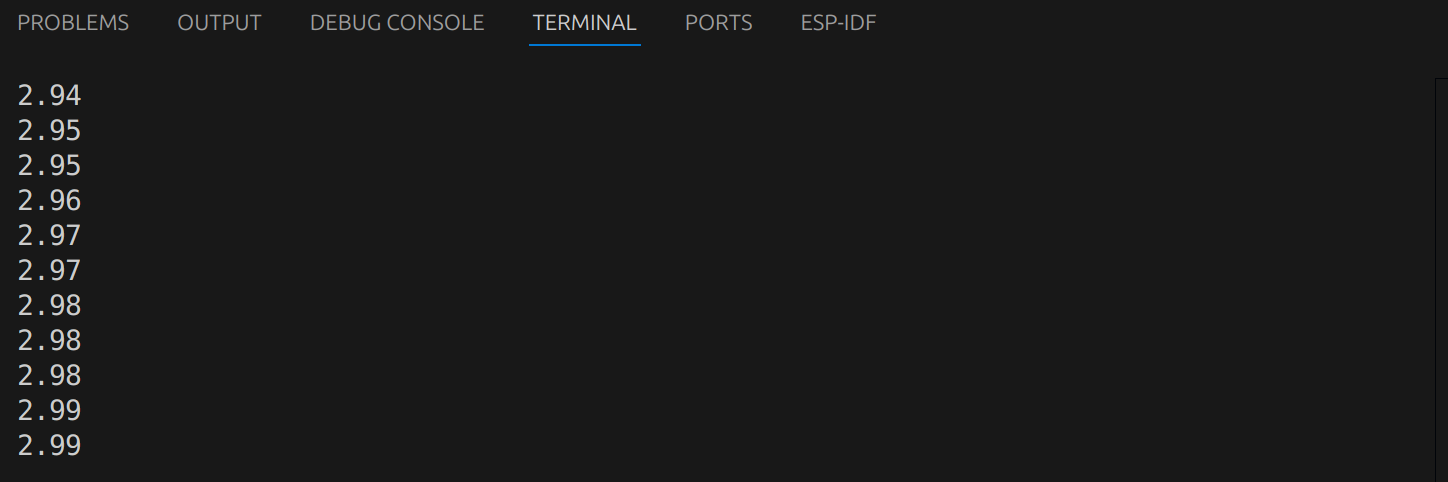
\includegraphics[width = 0.7\textwidth]{setup.png}
        \caption{Serial Output After Setup}
    \end{figure}
    \begin{minipage}{\textwidth}
        which states that I hav correctly set up the device in generating the Sine wave. 
    \end{minipage}\\[1em]
    \begin{minipage}{\textwidth}
        \Large
        \textbf{Setting up the PWM Signal:}
    \end{minipage}\\[0.5em]
    \begin{minipage}{\textwidth}
       1. When we are setting up the output on the SCL(D3), the timer we must use is the \textbf{Timer0/Counter0}. 
       2. Code for setting up the Fast PWM signal on the board:
       \begin{verbatim}
        // Timer Setup
        DDRD |= (1<<0);             // Set PD0 (Digital Pin 3) as output
        TCCR0A = 0b00100011;        // COM0B1:0 = 10 (non-inverting), 
                                       WGM01:00 = 11 (Fast PWM)
        TCCR0B = 0b00001011;        // WGM02 = 1 (Fast PWM with OCR0A as 
                                       TOP), CS02:00 = 011 (prescaler of 64)
        OCR0A = 124;                // Set TOP value for PWM
        OCR0B = 0;                  // Initialize duty cycle
       \end{verbatim}
       For \texttt{TCCR0A}, the selection si based on: 00 - Normal Port; 10 - Set 0A as the TOP; WGM11 for Fast PWM.\\
       For \texttt{TCCR0B}, I set the prescaler to 64 to make it easier to capture the diagram from the scope. \\
       For \texttt{OCR0A}, I set the value to 124 to make sure it is close to 1kHz when running while not surpassing it, as described in the lab manual.\\
       3. By using the Diligent Analog Discovery 2, I can have the PWM waveform generated by the board from the above code:
    \end{minipage}
    \begin{figure}[H]
        \centering 
        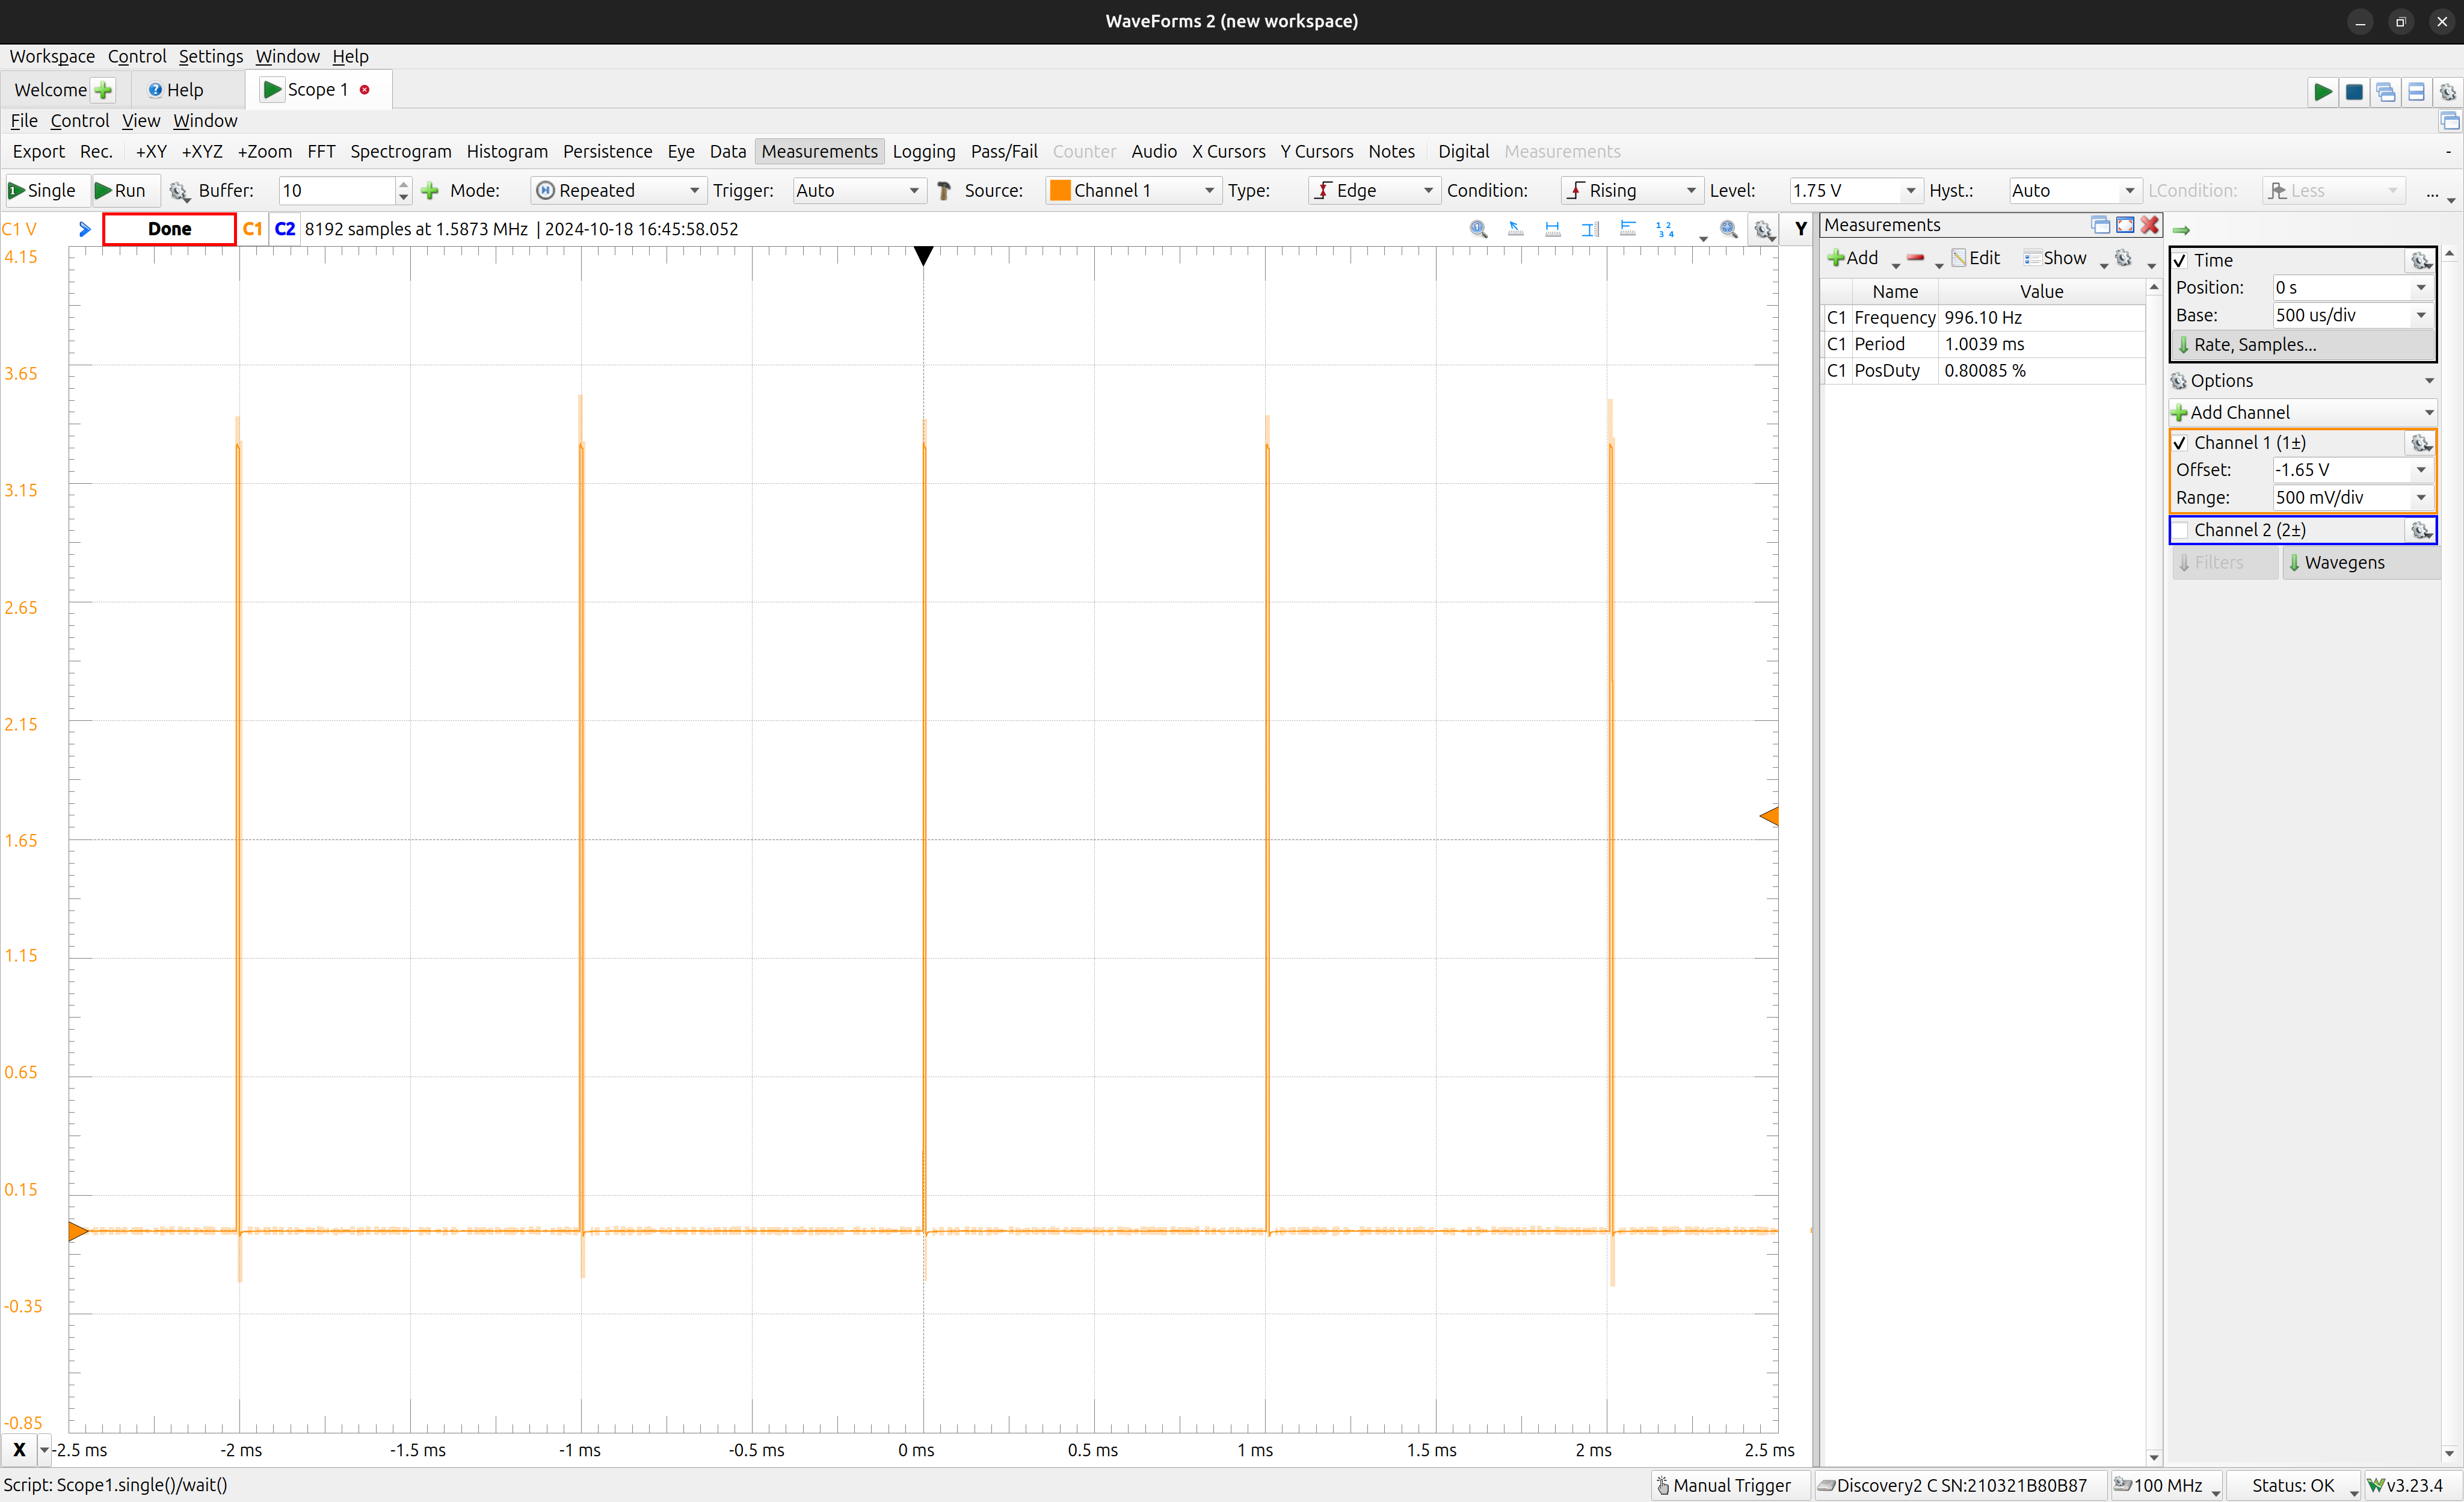
\includegraphics[width = 0.56\textwidth]{scope1.png}
        \caption{Scope After the PWM is set up}
   \end{figure}
   From the above diagram, we can see that the PWM is set to \textbf{\texttt{1kHz}}, as required in the manual. In order to make the duty cycle proportional to the value of the aval, I have added one line in the \texttt{loop()} function:
   \begin{verbatim}
    void loop() {
        // put your main code here, to run repeatedly:
        float aval;
        long x;
        x = millis();
        aval = abs(3 * sin(2 * 3.141592654 * x / 1000));
        OCR0B = (aval * OCR0A) / 3; // make the signal more discrete. 
        delay(1);
        Serial.println(aval);
    }
   \end{verbatim}
   After this modification, the output duty cycle changes as the value of \texttt{aval} changes:\\
   \begin{minipage}{0.49\textwidth}
    \begin{figure}[H]
    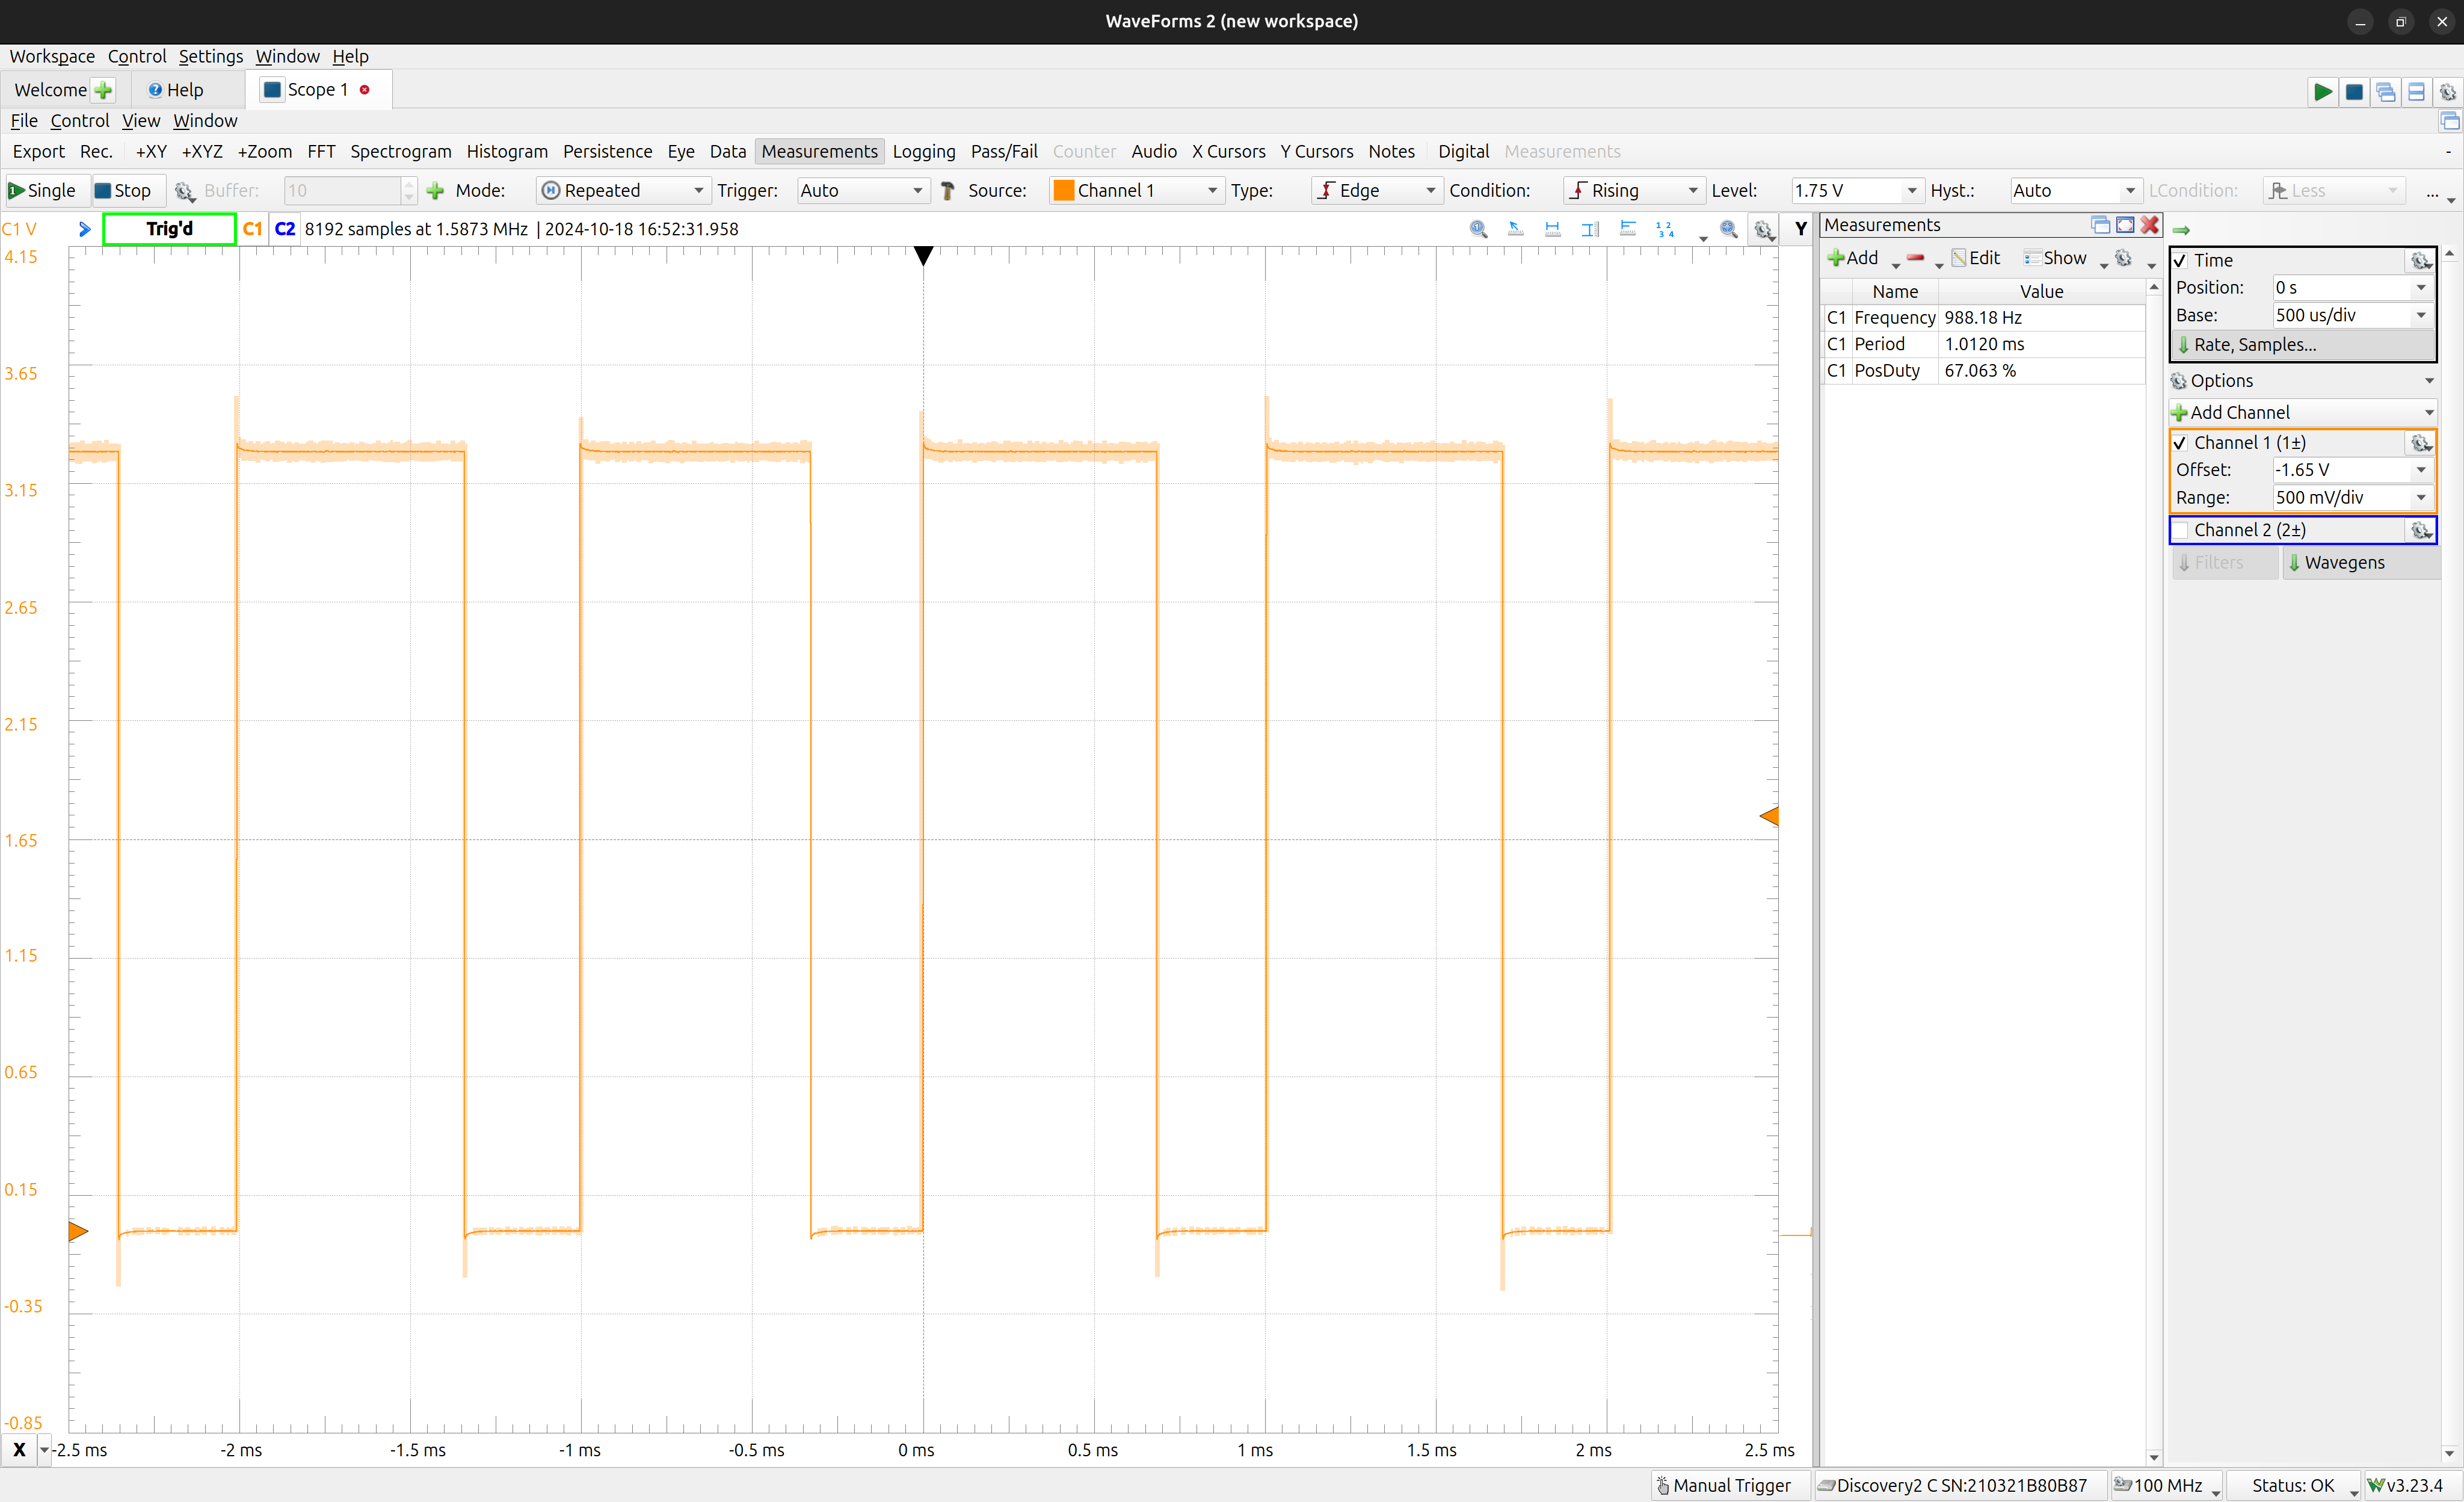
\includegraphics[width=\textwidth]{scope2.png}
    \caption{Scenario 1}
    \end{figure}
    \end{minipage}
    \hfill
    \begin{minipage}{0.49\textwidth}
        \begin{figure}[H]
        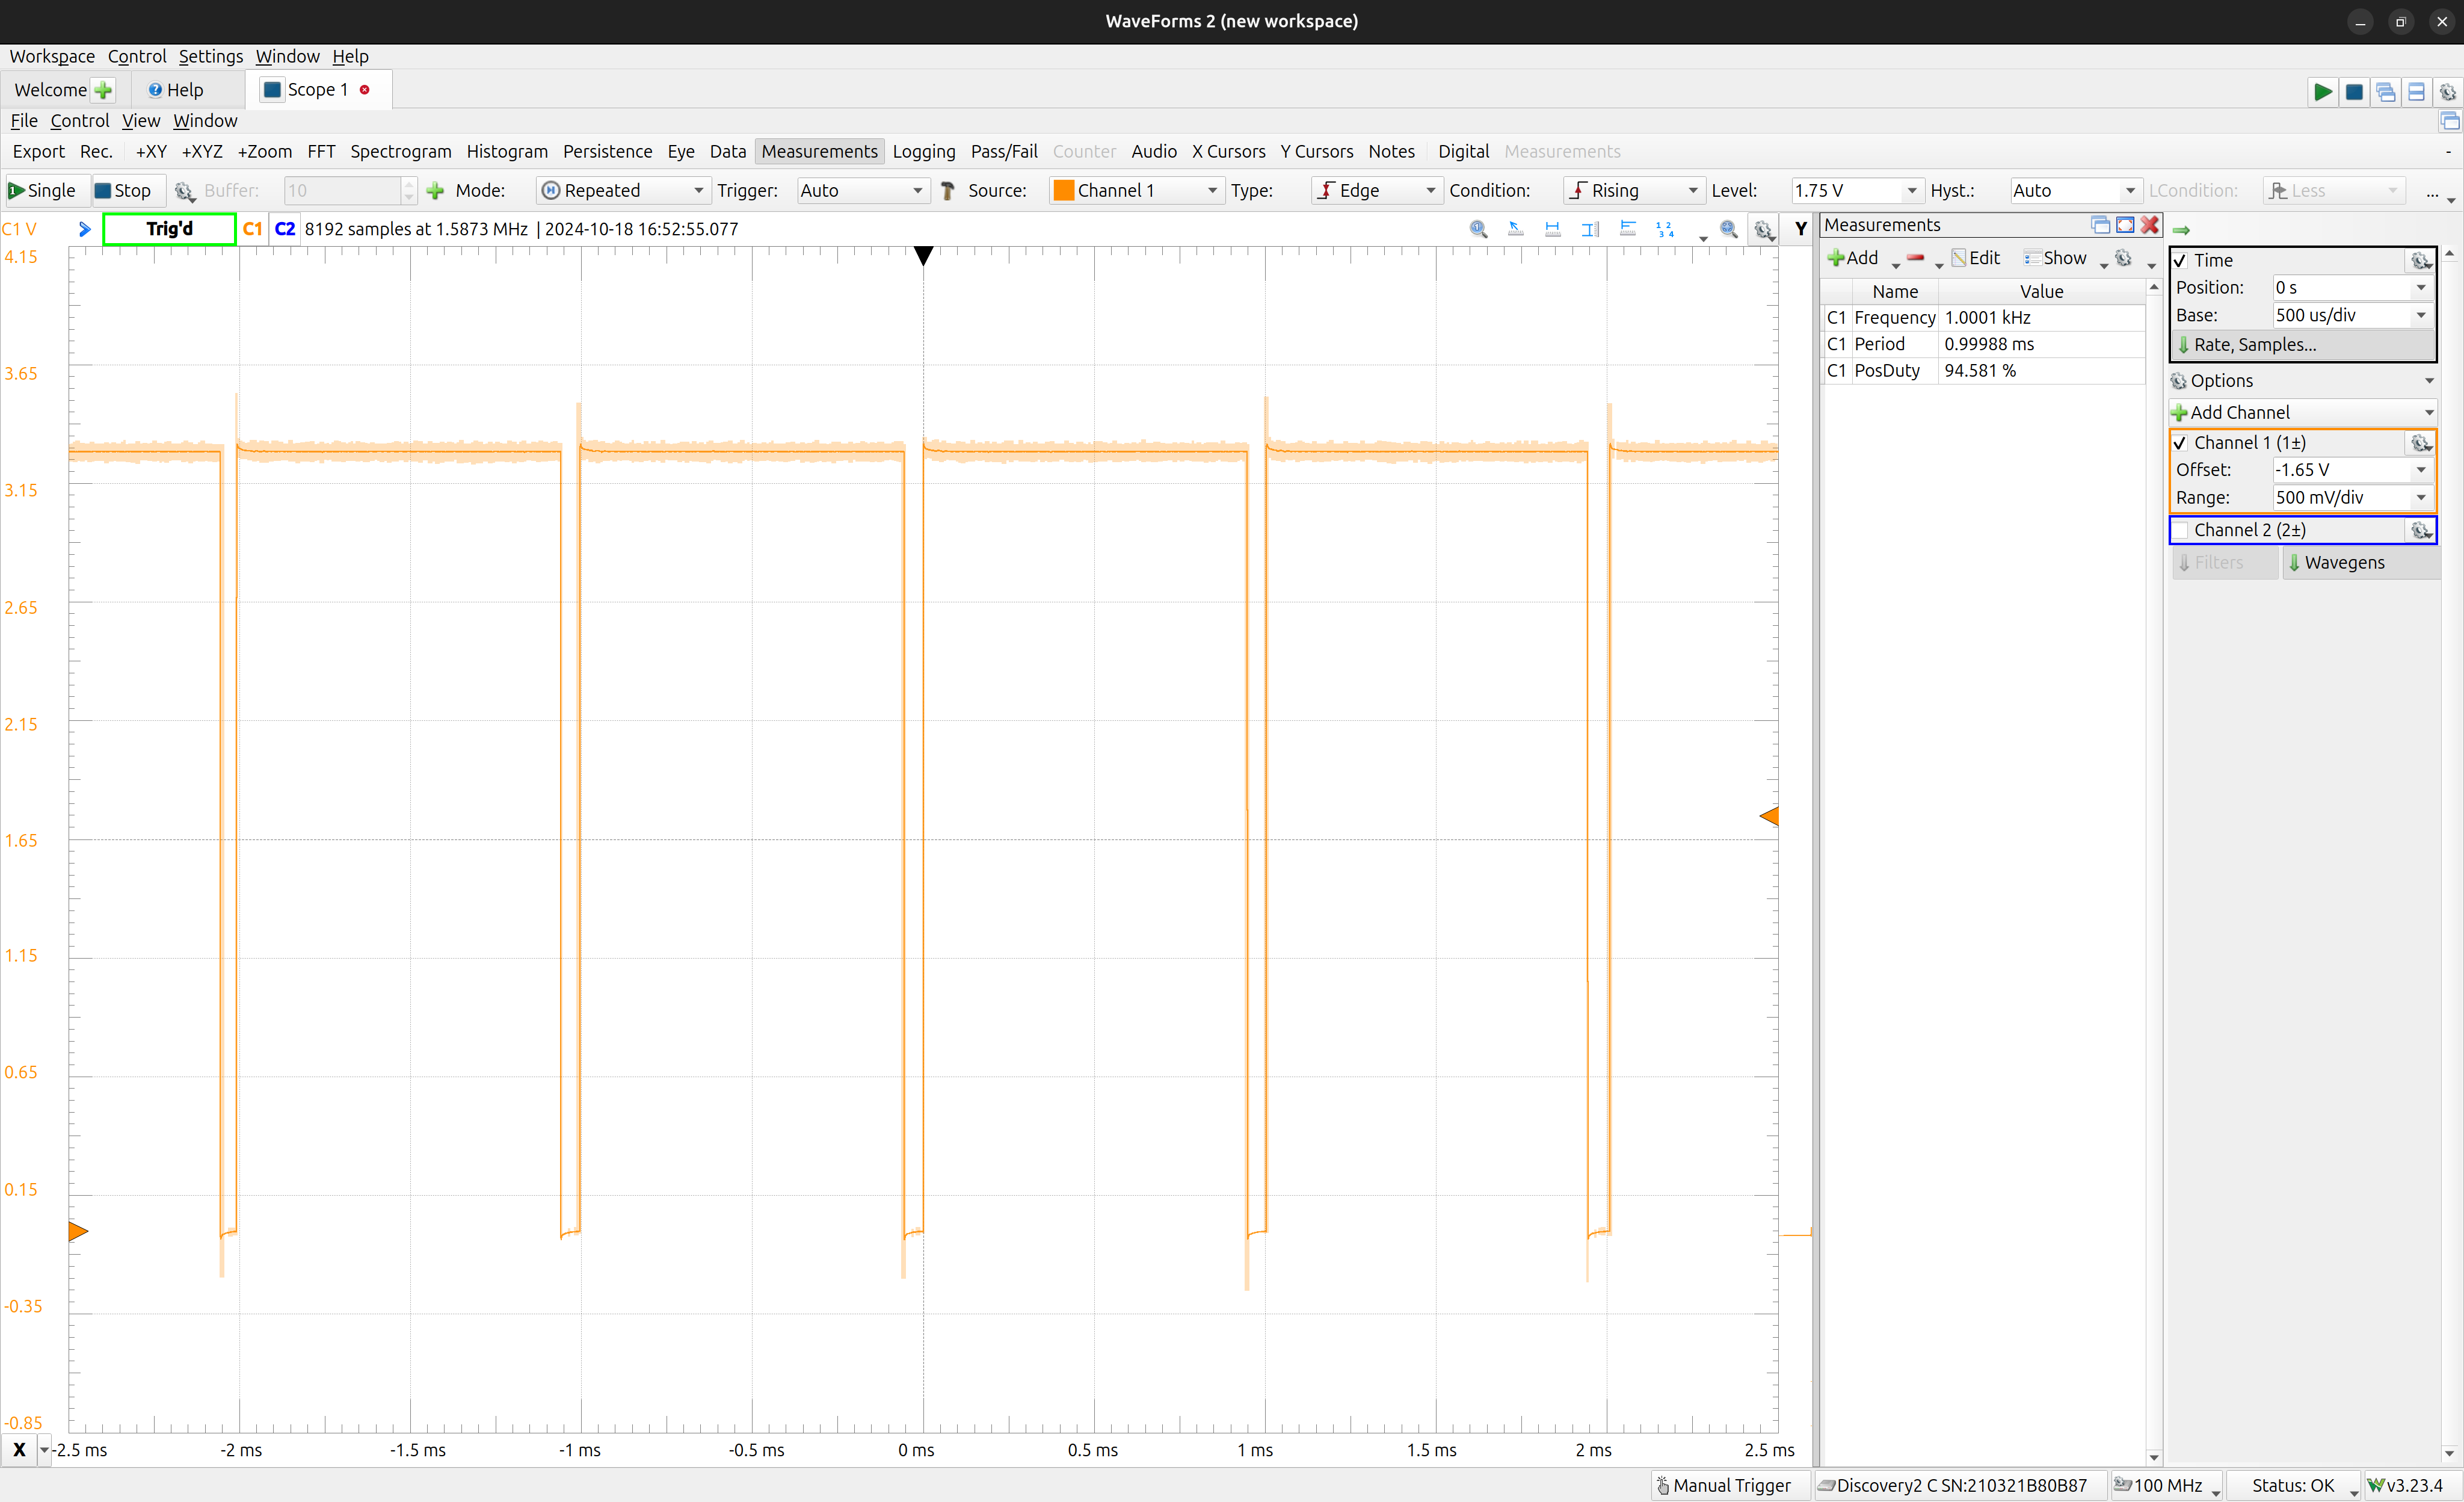
\includegraphics[width=\textwidth]{scope3.png}
        \caption{Scenario 2}
        \end{figure}
    \end{minipage}\\[0.5em]
    Now the PWM signal works just like the description in the manual, that the frequency is \textbf{1kHz} and the duty cycle changes as the \texttt{aval} changes. \\[1em]
    \begin{minipage}{\textwidth}
        \Large
        \textbf{Setting up the Demodulator:}
    \end{minipage}\\[0.5em]
    4. From the above diagram, we can see that the curren PWM signal frequency is 1kHz. From the code provided, we can see that the function generation is in milliseconds. Thus, the frequency should be 1Hz. The cutoff frequency, as described in the manual, should be:
    \begin{align*}
        \text{Frequency} &= \frac{1}{RC}\\
        &= \frac{1}{10K\Omega \cdot 1\mu F}\\
        &= 100Hz
    \end{align*}
    and we can see that PWM Signal $>$ Cutoff Frequency $>$ Analog Frequency, which is expected. 
    \begin{figure}[H]
        \centering
        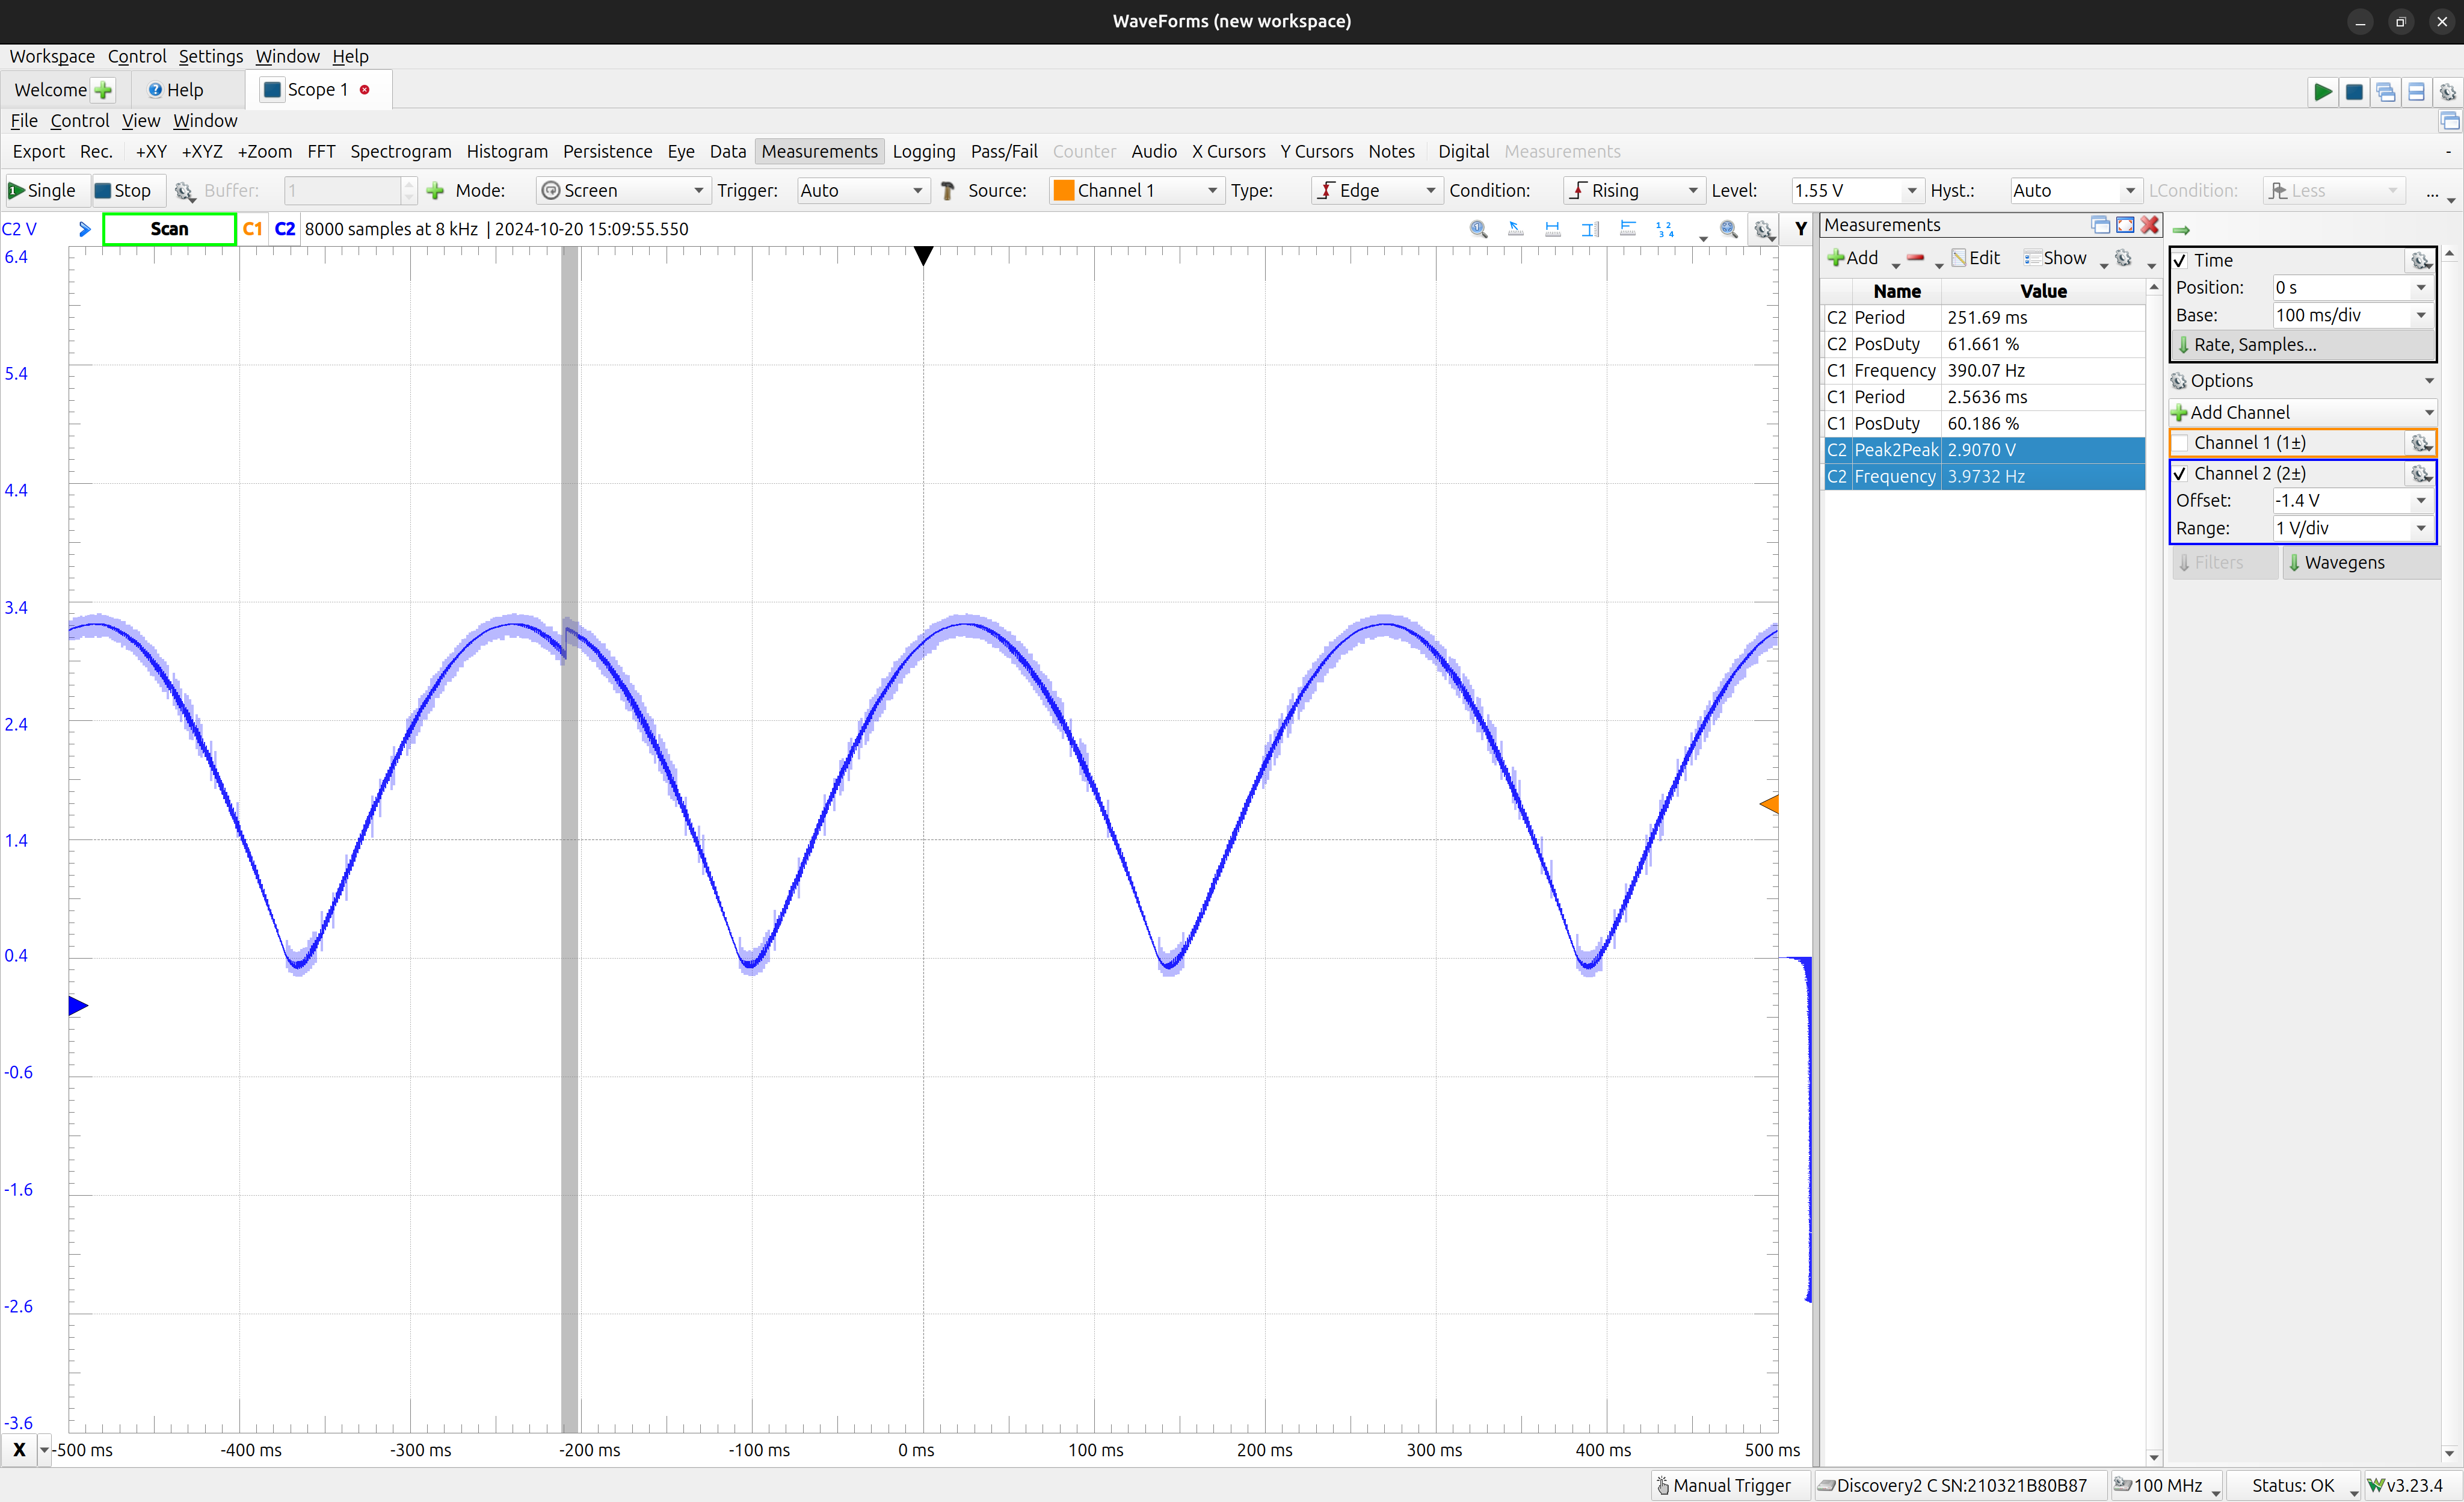
\includegraphics[width = 0.65\textwidth]{scope4.png}
        \caption{Scope After the Demodulator}
    \end{figure}
    From the above diagram, we can see that the analog output frequency is 4Hz, and the Peak to Peak value is around 3V. \\[1em]
    \begin{minipage}{\textwidth}
        \Large
        \textbf{Setting up the Analog Input:}
    \end{minipage}\\[0.5em]
    6. Now to set up the ADC on the board, I have the following code for registers:
    \begin{verbatim}
        // ADC Setup
        DDRD &= ~(1<<6);            // Set PD6 (ADC9) as input
        DIDR2 |= (1<<1);            // Disable digital input buffer on ADC9
        ADMUX = 0b01000001;         // REFS1:0 = 01 (AVCC), ADLAR = 0 (right adjust), 
                                       MUX4:0 = 00001 (ADC1 initially)
        ADCSRB = 0b00100000;        // MUX5 = 1 (for ADC8-ADC15), 
                                       ADTS2:0 = 000 (Free Running Mode)
        ADCSRA = 0b10100111;        // ADEN = 1 (enable ADC), ADATE = 1 (auto trigger), 
                                       ADPS2:0 = 111 (prescaler 128)
        ADCSRA |= (1<<ADSC);        // Start ADC conversions
    \end{verbatim}
    Now since the ADLAR selected above is 0, the code in the \texttt{loop()} is:
    \begin{verbatim}
        unsigned short *ADCData;
        unsigned short ADCVal;
        ADCData=(unsigned short *)0x78;
        ADCVal=(*ADCData & 0x3FF);

        float fADCVal;
        fADCVal=((float)ADCVal)/1023 * 3;
        Serial.print(abs(aval));

        Serial.print(" ");
        Serial.println(fADCVal);
        //Original rectified sinusoid
        //Analog voltage measured from ADC
    \end{verbatim}
    7. With the above codes in the \texttt{loop()} function, I got the following results in the serial portal in the PlatformIO:
    \begin{figure}[H]
        \centering
        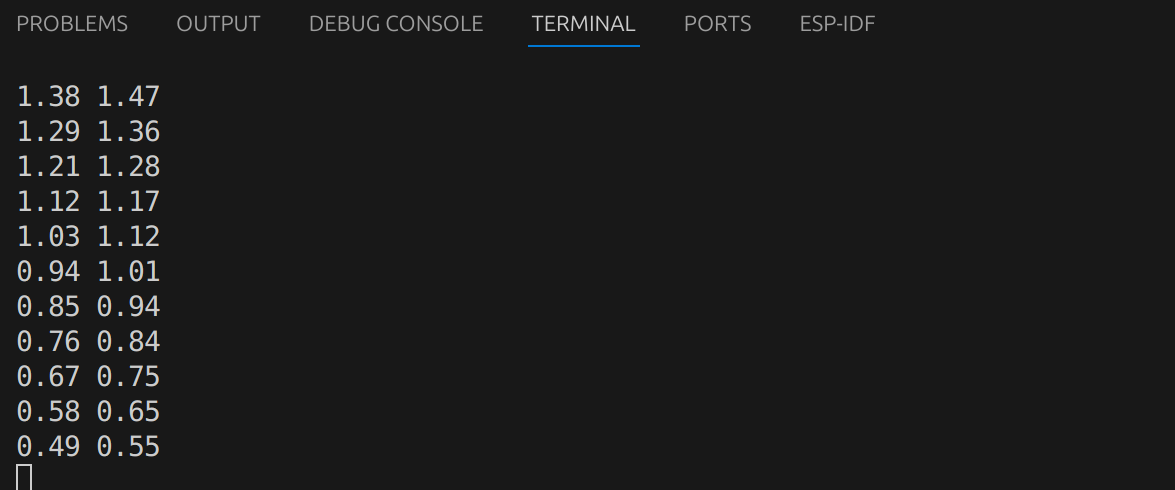
\includegraphics[width = 0.8\textwidth]{scope5.png}
        \caption{Serial Portal Output From the ADC}
    \end{figure}
\end{document}